% CVPR 2026 Paper Template; see https://github.com/cvpr-org/author-kit

\documentclass[10pt,twocolumn,letterpaper]{article}

%%%%%%%%% PAPER TYPE
\usepackage[review]{cvpr}

% Import additional packages in the preamble file, before hyperref
%% This file contains a number of tweaks that are typically applied to the main document.
%% They are not enabled by default, but can be enabled by uncommenting the relevant lines.


%%
%% Official support for 2-column teaser figure
%%
\usepackage{cuted} %< for strip environment

%%
%% For auto-referencing of figures (see fig/teaser.tex and \label{} therein) 
%%
% \usepackage{currfile} %< for \currfilebase macro

%%
%% caption and (global) spacing overrides
%%
\usepackage{caption} %< for "\captionof" commands (teaser)
% \setlength{\abovecaptionskip}{.5em} % space above caption
% \setlength{\belowcaptionskip}{1em} % space below caption

%%
%% Inline annotations; for predefined colors, refer to "dvipsnames" in the xcolor package:
%% https://tinyurl.com/overleaf-colors
%%
\newcommand{\red}[1]{{\color{red}#1}}
\newcommand{\todo}[1]{{\color{red}#1}}
\newcommand{\TODO}[1]{\textbf{\color{red}[TODO: #1]}}
%%
%% Disable for camera ready / submission by uncommenting these lines:
%%
% \renewcommand{\TODO}[1]{}
% \renewcommand{\todo}[1]{#1}

%%
%% Work harder in optimizing text layout. Typically shrinks text by 1/6 of page, enable
%% it at the very end of the writing process, when you are just above the page limit.
%%
% \usepackage{microtype}

%%
%% Fine-tune paragraph spacing.
%%
% \renewcommand{\paragraph}[1]{\vspace{.5em}\noindent\textbf{#1.}}

%%
%% Globally adjusts space between figure and caption.
%%
% \setlength{\abovecaptionskip}{.5em}

%%
%% Allows "the use of \paper to refer to the project name"
%% with automatic management of space at the end of the word.
%%
% \usepackage{xspace}
% \newcommand{\paper}{ProjectName\xspace}

%%
%% Commonly used math definitions.
%%
% \DeclareMathOperator*{\argmin}{arg\,min}
% \DeclareMathOperator*{\argmax}{arg\,max}

%%
%% Tighten underline.
%%
% \usepackage{soul}
% \setuldepth{foobar}

%%
%% Reconfigure paragraph (tweaks spacing)
%%


\definecolor{cvprblue}{rgb}{0.21,0.49,0.74}
\usepackage[pagebackref,breaklinks,colorlinks,allcolors=cvprblue]{hyperref}

%%%%%%%%% PAPER ID - UPDATE FOR THE SUBMISSION
\def\paperID{*****}
\def\confName{CVPR}
\def\confYear{2027}

%%%%%%%%% TITLE
\title{Joint Role--View Specialization for Training-Free Open-Vocabulary Remote Sensing Segmentation}

%%%%%%%%% AUTHORS - UPDATE FOR THE SUBMISSION
\author{First Author\\
Institution\\
Address\\
{\tt\small firstauthor@example.org}
}

\begin{document}

\maketitle

\begin{strip}
\centering
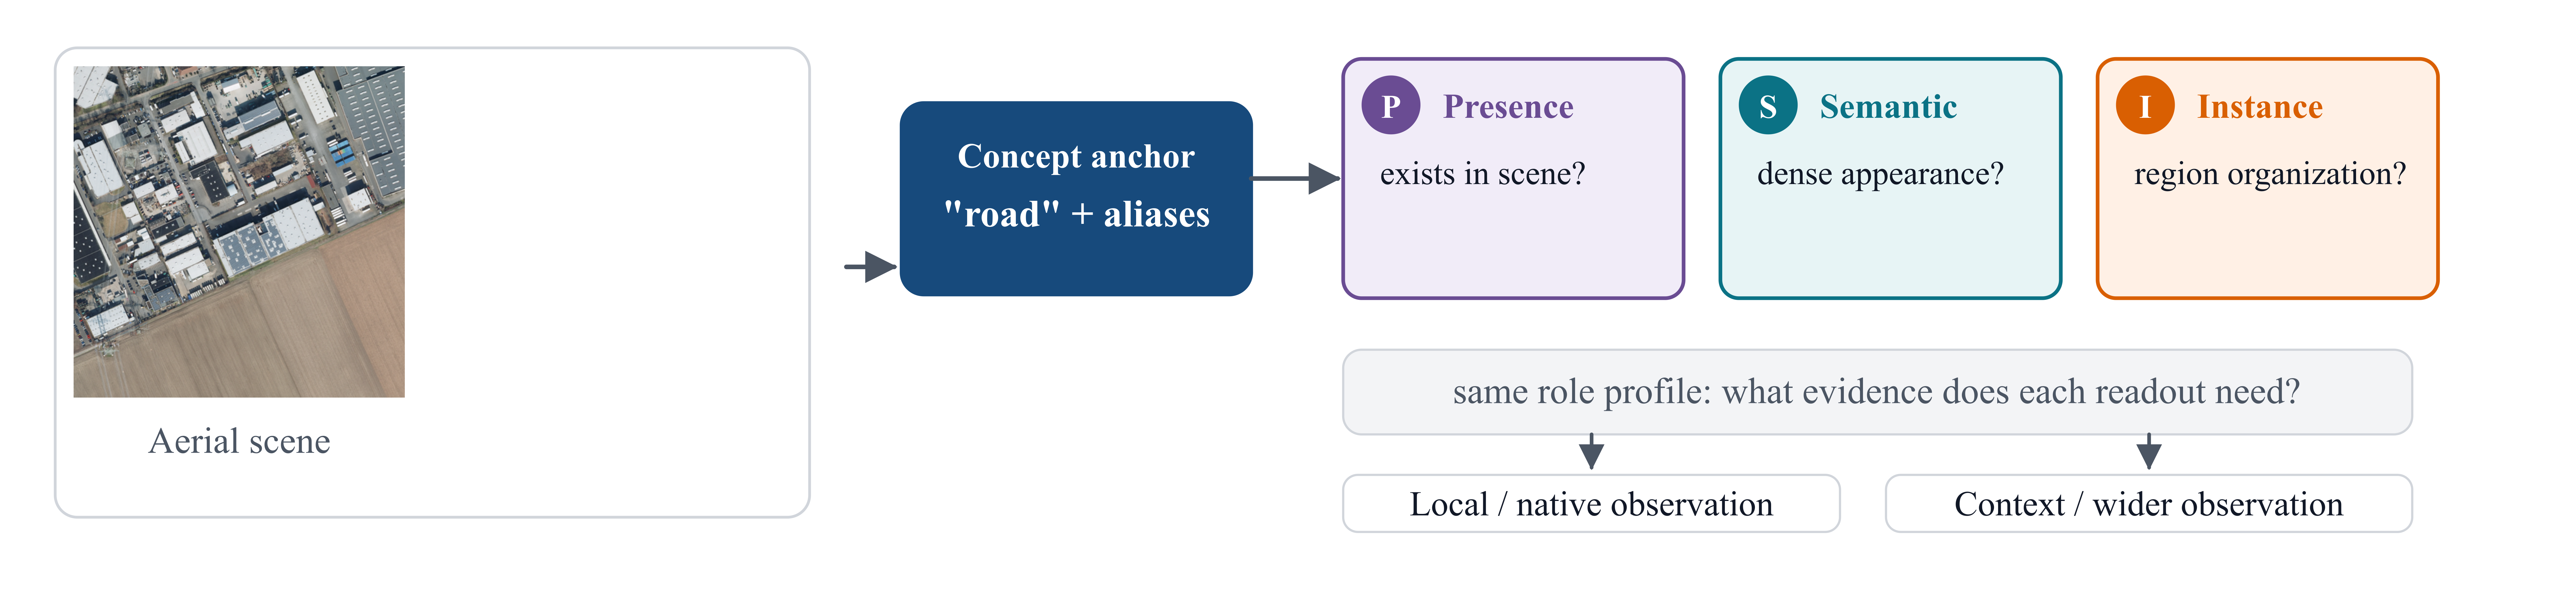
\includegraphics[width=\linewidth]{fig/intro_teaser.png}
\captionsetup{hypcap=false}
\captionof{figure}{Motivation. A shared concept anchor conditions three readouts with different evidence needs. The same selected role profile is evaluated under aligned Local and Context observations. The aerial image is illustrative.}
\label{fig:motivation}
\captionsetup{hypcap=true}
\end{strip}


\begin{abstract}
Training-free open-vocabulary semantic segmentation must assign arbitrary textual categories to dense remote-sensing imagery without updating the segmentation model. Concept-grounded segmenters such as SAM3 and SegEarth-OV3 provide a shared grounding state with distinct Presence, Semantic, and Instance readouts, but current methods typically condition all readouts with one category-level description and one visual observation. We study the resulting mismatch between shared concept grounding and heterogeneous evidence requirements. We introduce Joint Role--View Specialization (JRV), which preserves the official class anchor, grounds role-functional candidates with the complete frozen model, and applies bounded role-specific corrections while retaining the native Presence--Instance coupling. JRV then grounds spatially aligned Local and Context observations, reuses the same role profile across both views, and composes their complete class-score fields before the original class decision. On eight remote-sensing benchmarks, JRV raises the matched average mIoU from 53.56 to 57.49 and improves every dataset over the baseline. A matched Role--View factorial analysis shows positive interaction on six of eight datasets, while the natural-image evaluations show transfer of role supplementation and the dataset dependence of view composition. These results support organizing supplementary evidence by readout responsibility and observation condition rather than treating additional text or larger visual fields as uniformly beneficial. Our code is available at \url{https://github.com/pengjunhao621-arch/SegEarth3}.
\end{abstract}


% The Chinese counterpart is maintained at ../中文论文/论文中文版.md.
% References are fixed in R01--R51 order in references.tex to match the Chinese manuscript.
% Keep main.bib synchronized as source metadata.
% Future English sections should follow the section order in that file.

\section{Introduction}
\label{sec:introduction}

Open-vocabulary semantic segmentation (OVSS) assigns every pixel a category specified at inference time. Training-free methods adapt vision-language models to dense prediction \cite{R01,R06}. SAM3 instead conditions a shared grounding state on a text concept and exposes three readouts: Presence determines whether the concept occurs, Semantic estimates dense extent, and Instance organizes query-based regions \cite{R10}. SegEarth-OV3 applies this interface to remote sensing \cite{R11}. The shared state stabilizes category semantics, but the readouts need different evidence. In overhead scenes, small objects, continuous land cover, and scene-level existence are not captured equally well by one observation, and SAM3 presence and localization do not always improve together \cite{R24}. Figure~\ref{fig:motivation} summarizes this evidence-allocation problem.

Most existing methods adapt prompts or combine complete outputs. TMPA adjusts CLIP text embeddings \cite{R08}; ConceptBank evaluates candidate concepts with a support set \cite{R09}; ProC-SAM3 and CoCo-SAM3 fuse prompt-level evidence \cite{R12,R13}; RSGPNet refines SAM3 localization with geometric prompts \cite{R25}. A phrase is re-grounded through the full model, so it can improve dense coverage while changing presence or query organization. Replacing official class names also moves the ontology anchor. These methods operate at the category level even when their outputs affect several readouts.

Visual evidence imposes a second constraint. Local crops preserve detail but can cut long-range structure, whereas wider context exposes layout while undersampling small objects. Multi-resolution, cross-window, stitching, and scene-level inference methods exploit this complementarity \cite{R14,R15,R18,R26}, usually by changing attention, features, or a fixed fusion rule. For role-specific supplementation, the value of an observation also depends on which readout needs the missing evidence.

We introduce Joint Role--View Specialization (JRV). JRV keeps official names and aliases as an anchor, grounds role-functional candidates through the complete frozen SAM3 model, and applies only bounded corrections to their assigned readouts while preserving native Presence--Instance coupling. It then grounds aligned Local and Context observations with the same role profile and composes complete class-score fields before the original class decision. JRV does not modify SAM3 attention or give each head a separate visual path.

Our contributions are as follows:
\begin{itemize}[leftmargin=1.2em,itemsep=1pt,topsep=2pt]
  \item \textbf{Readout-level concept adaptation.} We introduce anchor-preserving Role-Functional Text. Supplementary descriptions are fully grounded, then used according to the responsibilities of Presence, Semantic, and Instance without replacing the official ontology or breaking Presence--Instance coupling.
  \item \textbf{Joint role--view specialization.} We treat role text and visual observation as joint conditions. One selected profile is reused across aligned Local and Context observations, and complete class-score fields are composed before argmax.
  \item \textbf{Evidence and scope.} On eight remote-sensing benchmarks, matched average mIoU rises from 53.56 to 55.82 with Role-only and 57.49 with Joint specialization. All datasets improve over the baseline, and six show positive Role--View interaction. Cityscapes and VOC20 test transfer and show that view composition remains distribution dependent.
\end{itemize}


\section{Related Work}
\label{sec:related_work}

\subsection{From OVSS to Concept Grounding}

Vision-language pretraining specifies categories through text rather than a fixed classifier \cite{R01}. Early open-vocabulary models learn text-supervised grouping or adapt masked regions to CLIP, as in GroupViT \cite{R45} and OVSeg \cite{R46}. Training-free dense methods subsequently reorganize pretrained CLIP representations: SCLIP modifies self-attention \cite{R29}, ClearCLIP decomposes final-layer representations \cite{R30}, ProxyCLIP injects spatial proxy attention from a vision foundation model \cite{R31}, and ResCLIP reuses residual cross-correlation attention \cite{R47}. Trained dense predictors instead learn cost aggregation or encoder--decoder fusion, as in CAT-Seg \cite{R48} and SED \cite{R49}. Applying these representations to segmentation still requires category semantics at dense spatial resolution. Training-free label propagation moves class evidence across patches and pixels \cite{R02}; CASS transfers object--context structure through spectral graph matching \cite{R03}; PEARL combines attention-space alignment with text-aware propagation \cite{R04}. Other trained approaches improve region--text correspondence or cost aggregation, as in Mask-Adapter \cite{R05} and PCA-Seg \cite{R17}. These methods improve the spatial usability of a shared vision-language representation, but the intervention remains at the level of representation, matching, or aggregation.

Remote sensing adds variation in object scale, appearance, and dataset ontology. SegEarth-OV adapts CLIP through feature upsampling and global-bias mitigation \cite{R06}. ReAttnCLIP reorganizes patch and global-token attention \cite{R07}. ReSeg-CLIP uses hierarchical SAM-mask constraints and remote-sensing CLIP composition \cite{R28}. DinoSplat-OV combines DINOv3/DINO.txt propagation with test-time upsampling \cite{R27}. RSGPNet converts coarse SAM3 text masks into geometric prompts and verifies cross-scale consistency \cite{R25}. SkySense-O builds a vision-centric model through remote-sensing pretraining \cite{R21}. These methods address domain shift, prompt localization, or representation combination, generally within a unified prediction. Our work starts from a frozen concept-grounded baseline and studies how evidence should be used by different native readouts after grounding.

\subsection{Concept and Prompt Adaptation}

Textual equivalence does not guarantee equivalent visual grounding. SynCLIP studies spatial inconsistencies across synonymous expressions \cite{R20}. TMPA generates context-aware descriptions and adapts CLIP text embeddings using high-confidence visual evidence and test-time entropy optimization \cite{R08}. ConceptBank builds visual prototypes from labeled support regions and evaluates concepts by their induced segmentation quality \cite{R09}. Promptable Concept Segmentation from Above evaluates zero-shot and one-shot SAM3 in overhead imagery and identifies a gap between concept presence and localization \cite{R24}. AVION verifies LLM-generated aerial descriptions with visual prototypes and distills them into prompt-tuned encoders \cite{R50}; it therefore involves training. The Power of Prior uses LLaVA-derived spatial priors to guide SAM prompts without task-specific fine-tuning \cite{R51}. These approaches implement category adaptation through candidate generation, embedding updates, or support prototypes, and their adaptation unit remains primarily the category or concept.

SAM3 turns text prompts into shared concept grounding and exposes category presence and spatial masks through a presence head and segmentation readouts \cite{R10}. SegEarth-OV3 organizes its semantic, instance, and presence outputs for remote-sensing OVSS \cite{R11}. ProC-SAM3 constructs a constrained prompt pool and adds a gated nonnegative instance advantage to a semantic base \cite{R12}. CoCo-SAM3 aggregates synonymous concept evidence and calibrates competition among independently prompted categories \cite{R13}. ActiveSAM keeps SAM3 frozen and restricts full-resolution decoding to an image-conditioned active vocabulary \cite{R35}; it targets inference efficiency and vocabulary pruning rather than readout-specific evidence allocation. These methods improve prompt coverage, inference efficiency, concept boundaries, or output fusion. We retain the official category anchor and complete grounding, allocate supplementary text according to the computational roles of Presence, Semantic, and Instance, and configure these roles jointly with visual observations. The closest comparator, ProC-SAM3, performs prompt-level fusion on a semantic base. Our distinction is readout-specific evidence use.

\subsection{Visual Observations and Context}

Detail and context form a basic trade-off in dense prediction. HRDA combines high-resolution detail crops with lower-resolution context predictions through learned scale attention \cite{R18}. SegMAN models multi-scale contextual dependencies within one segmentation network \cite{R23}, and F2Net uses frequency decomposition for ultra-high-resolution remote-sensing segmentation \cite{R19}. In training-free open-vocabulary segmentation, GLA-CLIP extends cross-window attention keys and values to exchange global information \cite{R14}. OV-Stitcher stitches cross-window Q/K/V and incorporates class-biased text prompts \cite{R15}. ConInfer aggregates scene and tile features and calibrates predictions through iterative consensus \cite{R26}. DPSeg uses visual prompts alongside text in cost-volume learning \cite{R16}, while MM-OVSeg obtains complementary evidence from registered optical and SAR imagery \cite{R22}. These works show that context and multimodal observations provide useful evidence, and fusion generally occurs in pretrained attention, a feature space, or a fixed output rule.

We use neither an auxiliary modality nor a modified SAM3 attention operator. For the same target region, we construct spatially aligned Local and Context observations from RGB data, ground each observation with the same frozen SAM3 model, and reuse one selected role profile across both. Their complete class-score fields are then composed in the target coordinate system. The resulting question is how role-specific textual supplementation changes the value of a visual observation and when the two form complementary evidence. GLA-CLIP and OV-Stitcher already combine context with text for training-free OVSS. Our distinction lies in jointly organizing evidence across native SAM3 readout responsibilities and observation conditions, not in context or text--vision collaboration itself.



\section{Method}
\label{sec:method}

\subsection{Preliminaries: Native Concept Grounding}

Given an RGB image $X$ and a set of class concepts $\mathcal C$, open-vocabulary semantic segmentation assigns each evaluated pixel a class in $\mathcal C$, with background determined by the benchmark protocol. For class $c$ and its text concept $t_c$, SegEarth-OV3 uses SAM3 to form a condition-dependent state \cite{R10,R11}:
\begin{equation}
H_c=\Phi(X,t_c).
\label{eq:state}
\end{equation}
The state supports three native readouts: a class-level Presence score $p_c$, a dense Semantic map $S_c(x)$, and an Instance map assembled from object-query masks. For query $q$, let $M_{cq}(x)$ be its mask value at pixel $x$ and $r_{cq}$ its raw object confidence. Let $\eta$ be the query-admission threshold and $a_c$ the admission score. The native implementation uses $a_c=p_c$; an anchor-admission variant described below uses the anchor Presence instead. The admitted queries and instance map are
\begin{equation}
\begin{aligned}
Q_c&=\{q:a_c r_{cq}>\eta\},\\
I_c(x)&=\max_{q\in Q_c}M_{cq}(x)r_{cq}p_c.
\end{aligned}
\label{eq:instance}
\end{equation}
Semantic and instance evidence are combined by the native chain
\begin{equation}
F_c(x)=p_c\max\bigl(S_c(x),I_c(x)\bigr).
\label{eq:native-fusion}
\end{equation}
Presence therefore acts on query admission, instance amplitude, and final class scaling. The class maps are compared by pixel-wise argmax, and the baseline threshold assigns low-confidence pixels to background. For a class with aliases, the official path aggregates the prompt-wise outputs in its original order. We denote the resulting single-observation class-score map by $G^{\mathrm{o}}$.

\begin{figure*}[!t]
\centering
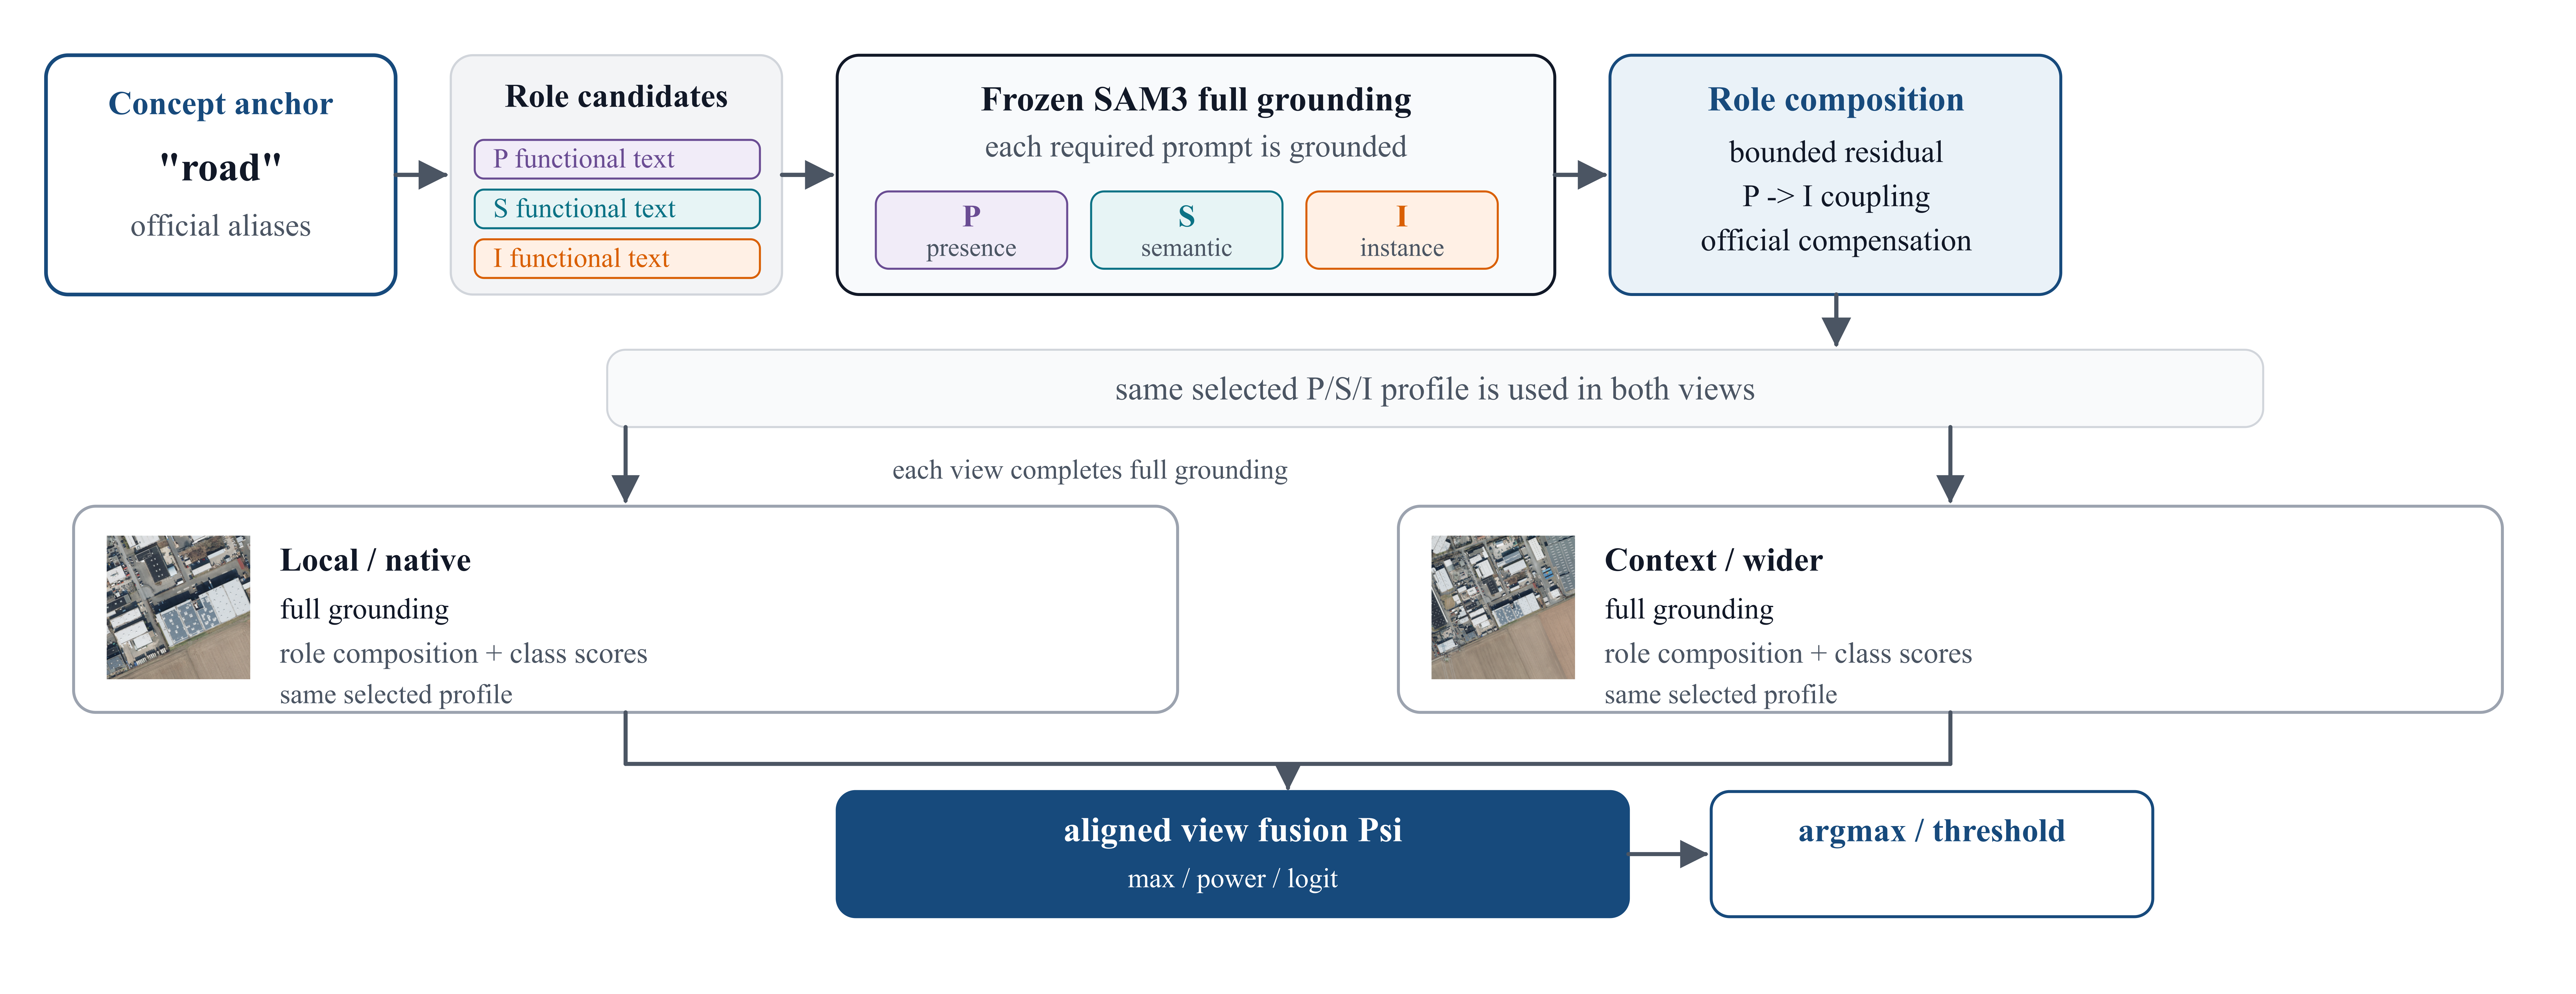
\includegraphics[width=\linewidth]{fig/method_overview.png}
\caption{Overview of Joint Role--View Specialization. Each required prompt is fully grounded by the frozen model. The same selected role profile is applied in Local and Context observations, and complete class-score fields are fused before the original class decision.}
\label{fig:method-overview}
\end{figure*}

 Figure~\ref{fig:method-overview} summarizes the complete evidence path.

\subsection{Role-Functional Text}

The official class name and aliases define an ontology anchor. We keep their native outputs as $(p_c^A,S_c^A,I_c^A)$ and build a small, frozen candidate bank for each class. Presence candidates describe how the concept is established or visible in a scene; Semantic candidates describe dense appearance, surface, coverage, and continuity; Instance candidates describe the organization and separation of query-supported regions. A zero slot keeps the anchor for that role, so not every class requires a non-anchor phrase.

Each non-anchor candidate is grounded through the complete frozen SAM3 model, producing $(p_c^r,S_c^r,I_c^r)$ for $r\in\{P,S,I\}$. We do not route a candidate directly into an isolated head. The assigned readout is combined with its anchor through a bounded residual. For two scalar or spatial quantities $a$ and $b$, define
\begin{equation}
\mathcal B(a,b)=\operatorname{clip}_{[0,1]}\!\left(a+\alpha\,\operatorname{clip}(b-a,-\tau,\tau)\right),
\label{eq:bounded}
\end{equation}
with $\alpha=0.5$ and $\tau=0.25$ in the reported configuration. The Presence and Semantic updates are
\begin{equation}
\begin{aligned}
\tilde p_c&=\mathcal B(p_c^A,p_c^{\pi_P}),\\
\tilde S_c(x)&=\mathcal B(S_c^A(x),S_c^{\pi_S}(x)).
\end{aligned}
\label{eq:role-updates}
\end{equation}
Because Presence affects instance construction, the instance maps are rebuilt after the Presence update. With admission score $a$, the anchor and candidate instance maps are
\begin{equation}
\begin{aligned}
I_A^{\tilde p}&=\mathcal I(Q_A;\tilde p,a),\\
I_{\pi_I}^{\tilde p}&=\mathcal I(Q_{\pi_I};\tilde p,a),\\
\tilde I_c&=\mathcal B(I_A^{\tilde p},I_{\pi_I}^{\tilde p}),
\end{aligned}
\label{eq:instance-rebuild}
\end{equation}
where $\mathcal I$ denotes the query aggregation in Eq.~\eqref{eq:instance}. The role-composed class evidence is then
\begin{equation}
F_{\pi,c}(x)=\tilde p_c\max\bigl(\tilde S_c(x),\tilde I_c(x)\bigr).
\label{eq:role-final}
\end{equation}
For native admission, $a=\tilde p_c$; for anchor admission, only query membership uses $a=p_c^A$, while the amplitude and final scaling still use the updated Presence. If all role slots are zero, the updates reduce to the anchor.

The official score field is retained to preserve aliases and the baseline aggregation order. Let $G_v^{\mathrm{o}}$ be the official map for observation $v$, $F_{v,\pi}$ the role-composed map, and $F_v^A$ the anchor composition without supplementary text. The observation-level output is
\begin{equation}
G_{v,\pi}=\operatorname{clip}_{[0,1]}\!\left(G_v^{\mathrm{o}}+F_{v,\pi}-F_v^A\right).
\label{eq:official-compensation}
\end{equation}
Thus, disabling all role updates returns the official map exactly. The construction is not an ensemble of three independent predictions: candidates are re-grounded completely, only their assigned readout changes the anchor, and the native Presence--Instance coupling remains active.

\subsection{Aligned Local and Context Observations}

A text description can specify a continuous surface or a complete region, but it cannot create visual evidence absent from the observation. Local observations preserve effective sampling density for boundaries and small objects; Context observations expose a wider spatial layout and long-range continuity. For datasets supplied as coordinate tiles, Context observations are assembled from spatially aligned neighboring RGB tiles without neighboring labels; otherwise they are enlarged crops of the input image. The evaluation protocol specifies the exact construction.

Every observation completes the native grounding and role composition independently. The Local and Context observations reuse the same selected role profile; JRV does not assign Presence to one view, Semantic to a second, or Instance to a third. For a view family $v\in\{L,G\}$ with target units $\mathcal U_v$, each unit $u$ produces a role-composed map $G_{u,\pi}$ on its own coordinate system. Let $W_u$ restore the map to the target coordinates and let $w_u(x)$ indicate valid coverage. The aligned view evidence is
\begin{equation}
\overline G_{v,c}(x)=
\frac{\sum_{u\in\mathcal U_v}w_u(x)\,W_u[G_{u,\pi,c}](x)}
{\sum_{u\in\mathcal U_v}w_u(x)}.
\label{eq:view-average}
\end{equation}
The final class-score field is
\begin{equation}
\begin{aligned}
Z_c(x)&=\Psi_{\omega}\!\left(\overline G_{L,c}(x),\overline G_{G,c}(x)\right),\\
\widehat Y&=\mathcal D_{\mathrm{base}}(Z),
\end{aligned}
\label{eq:view-fusion}
\end{equation}
where $\mathcal D_{\mathrm{base}}$ retains the baseline argmax and background threshold. The profile operator $\Psi_{\omega}$ is fixed rather than learned. We use element-wise maximum, Local or Context endpoints, weighted power means, and weighted logit fusion:
\begin{equation}
\begin{aligned}
\Psi_{\max}(L,G)&=\max(L,G),\\
\Psi_{\rho,g}(L,G)&=\left((1-g)L^{\rho}+gG^{\rho}\right)^{1/\rho}.
\end{aligned}
\label{eq:view-operators}
\end{equation}
The logit variant uses the same mixture in log-odds space:
\begin{equation}
\Psi_{\mathrm{logit},g}(L,G)=\sigma\!\left((1-g)\operatorname{logit}(L)+g\operatorname{logit}(G)\right).
\label{eq:logit-operator}
\end{equation}
The operator family is a profile choice, not a new learned attention module. Combining complete class-score fields preserves the native cross-category decision after role and view composition.

\begin{figure*}[!t]
\centering
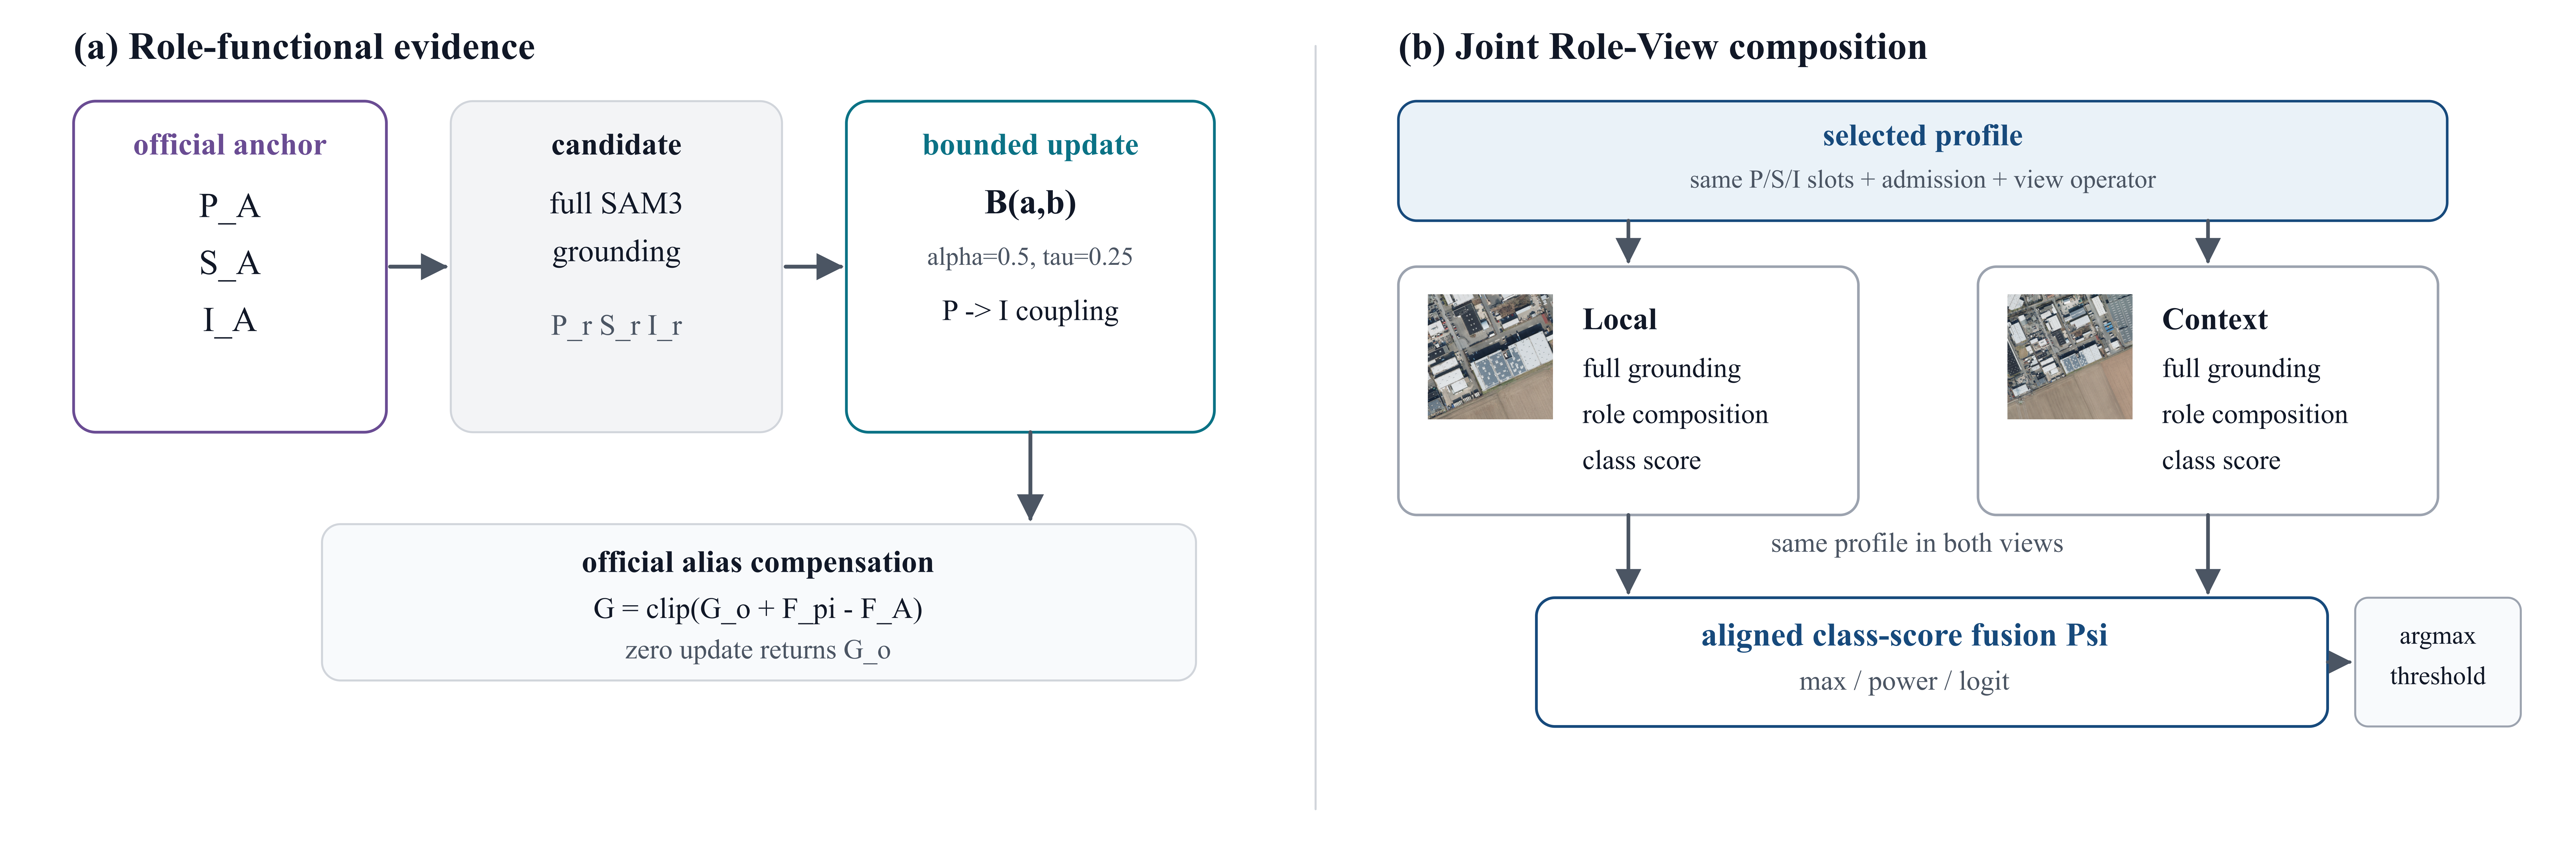
\includegraphics[width=\linewidth]{fig/method_detail.png}
\caption{Method details. (a) Role-functional evidence keeps the official anchor, applies bounded role updates, rebuilds Instance after the Presence update, and restores the official map through alias compensation. (b) Local and Context observations reuse the same profile and are fused after complete class-score composition.}
\label{fig:method-detail}
\end{figure*}

 Figure~\ref{fig:method-detail} isolates the two evidence interactions.

\subsection{Inference Protocol and Profile Definition}

A dataset profile is a fixed tuple
\begin{equation}
\pi=(s_P,s_S,s_I,a,\Psi_{\omega}),
\label{eq:profile}
\end{equation}
where each $s_r$ indexes a candidate slot in the frozen text bank, $s_r=0$ retains the anchor, $a$ specifies native or anchor admission, and $\Psi_{\omega}$ specifies the view operator. The same profile is applied to every image in a benchmark and to both Local and Context observations. The text bank and profile are fixed before inference; SAM3 weights are never updated. Profile selection is dataset-level and offline, and the experimental section reports the selection protocol. No image-level ground-truth routing is used.

Three implementation properties connect the method to the experimental analysis. Every required supplementary phrase undergoes full native grounding rather than modifying an isolated decoder state. An unchanged slot or an all-zero role profile recovers the anchor path, including the official alias aggregation. Local and Context outputs are combined only after complete role composition and coordinate restoration, so the method changes evidence use rather than SAM3 attention or its internal fusion operator.



\section{Experiments}
\label{sec:experiments}

\subsection{Experimental Setup}

We evaluate on the eight remote-sensing benchmarks used by SegEarth-OV and SegEarth-OV3 \cite{R06,R11}: Potsdam and Vaihingen \cite{R42}, LoveDA \cite{R36}, iSAID \cite{R37}, OpenEarthMap (OEM) \cite{R38}, UAVid \cite{R39}, UDD5 \cite{R40}, and VDD \cite{R41}. We retain the baseline evaluation splits, class mappings, ignored labels, and image-based UAVid protocol. iSAID contains 11,644 processed validation tiles, and UAVid contains 1,020 evaluated patches. The primary metric is mean intersection over union (mIoU, \%). The overall average weights the eight datasets equally. Class-group analysis weights dataset--class pairs equally and is reported separately. VOC20 \cite{R44} and Cityscapes \cite{R43} provide additional natural-image evaluations.

Potsdam and Vaihingen are ISPRS airborne urban benchmarks; LoveDA covers urban and rural land cover from three Chinese cities; iSAID is a large aerial instance-segmentation dataset derived from DOTA; OpenEarthMap is a global high-resolution land-cover benchmark; UAVid focuses on oblique UAV urban scenes; UDD5 is built from semantic-constrained aerial structure-from-motion; and VDD emphasizes varied drone scenes and flight conditions. VOC20 contains the 20 PASCAL VOC foreground classes, and Cityscapes provides 19-class urban street-scene evaluation.

All experiments and inference were conducted on four NVIDIA RTX 3090 GPUs. The SAM3 weights remained frozen, and no model training or fine-tuning was performed. Candidate descriptions are generated offline and stored verbatim. Unless stated otherwise, $\alpha=0.5$ and $\tau=0.25$. For each benchmark, the role slots, admission mode, and view operator are selected offline using the available evaluation annotations and then fixed for every image. Inference with a fixed profile does not access annotations. The reported results therefore use evaluation-selected dataset-level profiles, not an independent held-out configuration-selection split.

Local and Context observations are built from RGB data. For Potsdam and Vaihingen, the selected main protocol uses spatially aligned neighboring RGB tiles from the same original scene to reconstruct a 1,024-pixel context around a 512-pixel target; only the target region is scored, and neighboring ground truth is never used. This input extent is larger than the isolated-tile baseline. The same-image 256/512 control is reported as a scope experiment rather than a replacement for the main protocol. No temporal frames, labeled visual exemplars, or auxiliary sensing modalities are used.

Competitor values in Table~\ref{tab:main-comparison} are transcribed from the ProC-SAM3 comparison \cite{R12}; the reproduced SegEarth-OV3 row and JRV come from matched local runs. All component gains and interaction statistics use the full-precision matched baseline, not the one-decimal comparison table. The mixed provenance means that Table~\ref{tab:main-comparison} supports an internal numerical comparison, not an independently established leaderboard rank.


\begin{table*}[!t]
\centering
\captionsetup{hypcap=false}
\caption{Remote-sensing open-vocabulary semantic segmentation (mIoU, \%). Method and dataset names cite their original papers. Competitor metrics follow the comparison in ProC-SAM3 \cite{R12}; published values may correspond to the versions used there. The SegEarth-OV3 row is our reproduction, and JRV uses the context-access protocol in Section~\ref{sec:experiments}. Avg. is the equal-weight mean over eight datasets, and published values retain their reported precision.}
\captionsetup{hypcap=true}
\label{tab:main-comparison}
\setlength{\tabcolsep}{2pt}
\scriptsize
\begin{tabular}{lcccccccccc}
\toprule
Method & Backbone & Potsdam~\cite{R42} & Vaihingen~\cite{R42} & LoveDA~\cite{R36} & iSAID~\cite{R37} & OEM~\cite{R38} & UAVid~\cite{R39} & UDD5~\cite{R40} & VDD~\cite{R41} & Avg. \\
\midrule
VIP~\cite{R32} & DINOv3 + dino.txt & 23.0 & 30.5 & 31.2 & 23.5 & 20.7 & 19.9 & 35.2 & 52.5 & 29.6 \\
SCLIP~\cite{R29} & CLIP & 39.6 & 35.9 & 30.4 & 16.1 & 29.3 & 31.4 & 38.7 & 37.9 & 32.4 \\
ClearCLIP~\cite{R30} & CLIP & 42.0 & 36.2 & 32.4 & 18.2 & 31.0 & 36.2 & 41.8 & 39.3 & 34.6 \\
ProxyCLIP~\cite{R31} & CLIP + DINOv2 & 49.0 & 47.5 & 34.3 & 21.8 & 38.9 & 35.8 & 40.8 & 47.8 & 39.5 \\
SegEarth-OV~\cite{R06} & CLIP & 48.5 & 29.1 & 36.9 & 21.7 & 40.3 & 42.5 & 50.6 & 45.3 & 39.2 \\
RSCLIP~\cite{R33} & CLIP & 47.4 & 40.3 & 35.5 & 21.2 & 39.8 & 42.5 & 50.4 & 42.5 & 39.9 \\
CorrCLIP~\cite{R34} & CLIP + DINO + SAM2 & 51.9 & 47.0 & 36.9 & 25.5 & 32.9 & 38.3 & 46.1 & 47.3 & 40.7 \\
ConInfer~\cite{R26} & CLIP + DINOv3 & 50.0 & 31.4 & 39.3 & 20.1 & 42.0 & 46.4 & 46.9 & 50.3 & 40.8 \\
ReAttnCLIP~\cite{R07} & CLIP & 48.7 & 29.9 & 37.0 & 23.2 & 41.1 & 44.0 & 53.7 & 49.7 & 40.9 \\
ActiveSAM~\cite{R35} & SAM3 & 40.6 & 45.1 & 41.1 & 28.3 & 40.7 & 53.3 & 72.1 & 62.2 & 47.9 \\
SegEarth-OV3 (reproduced)~\cite{R11} & SAM3 & 57.8 & 60.8 & 47.4 & 27.6 & 44.3 & 54.7 & 71.7 & 64.1 & 53.5 \\
ProC-SAM3~\cite{R12} & SAM3 & 58.8 & 64.5 & 46.1 & \textbf{29.5} & 48.9 & \textbf{60.0} & \textbf{73.4} & \textbf{67.5} & 56.1 \\
JRV (ours) & SAM3 & \textbf{63.2} & \textbf{66.4} & \textbf{48.8} & 29.1 & \textbf{53.1} & 59.8 & 72.9 & 66.6 & \textbf{57.5} \\
\bottomrule
\end{tabular}
\end{table*}

\subsection{Comparison with Existing Methods}



JRV reaches 57.49 average mIoU in the full-precision pairwise evaluation. The matched baseline is 53.56, giving an average gain of 3.92 points. Role-Functional Text accounts for 2.25 points, and joint view composition adds another 1.67 over the independently selected best role-only stage. Gains appear on all eight datasets. The largest increases are on OEM (+8.77), Vaihingen (+5.52), Potsdam (+5.31), and UAVid (+5.24).

Against the reported ProC-SAM3 row, JRV is higher on four datasets and lower on four, with a 1.39-point higher displayed average. The comparison is useful for positioning because ProC-SAM3 is the strongest verified published result under the full eight-dataset, training-free protocol. It remains a mixed-source comparison, and we do not describe the internal 57.49 result as an independently established state of the art.

\subsection{Functional Use of Supplementary Text}

We first separate the two stages of the final system under a fixed inference recipe. Table~\ref{tab:component-progression} reports the macro progression over the eight benchmarks and establishes the language-evidence stage before the matched interaction analysis.

\begin{table}[!htbp]
\centering
\caption{Macro component progression. Stage entries refer to the configurations defined in Section~3; Role-only is the best recorded independent role profile and is not the matched Role condition used for interaction analysis.}
\label{tab:component-progression}
\small
\setlength{\tabcolsep}{3pt}
\begin{tabular}{lccc}
\toprule
Stage & Macro mIoU & $\Delta$ vs baseline & Positive \\
\midrule
Matched baseline & 53.56 & -- & -- \\
Role-Functional Text & 55.82 & +2.25 & 8/8 \\
Joint Role--View & 57.49 & +3.92 & 8/8 \\
\bottomrule
\end{tabular}
\end{table}

Across the sequence, Role-only improves every dataset over the matched baseline, including gains of 6.23 on OEM and 4.92 on UAVid. Joint composition then improves over the role-only stage on every dataset. The component progression therefore supports both the language-evidence stage and the additional view stage, while the interaction analysis below fixes the profile to avoid selecting a different role configuration for each cell.

We next hold the role slots and admission mode fixed and ask how the same semantic-oriented candidate should be used. Table~\ref{tab:role-use} compares Semantic-only supplementation with sharing that candidate across Presence, Semantic, and Instance.

\begin{table}[!htbp]
\centering
\caption{The same semantic-oriented candidate used either only for Semantic supplementation or for all three roles. Both variants retain the anchor and bounded update; values are final mIoU.}
\label{tab:role-use}
\footnotesize
\setlength{\tabcolsep}{2pt}
\begin{tabular}{llccc}
\toprule
Dataset & Candidate & Baseline & Semantic only & Shared P/S/I \\
\midrule
Potsdam~\cite{R42} & S2 & 57.87 & \textbf{58.00} & 56.63 \\
Vaihingen~\cite{R42} & S3 & 60.86 & \textbf{61.57} & 61.28 \\
LoveDA~\cite{R36} & S1 & 47.34 & \textbf{48.09} & 46.61 \\
OEM~\cite{R38} & S3 & 44.30 & \textbf{46.28} & 44.02 \\
UDD5~\cite{R40} & S3 & 71.80 & 71.56 & \textbf{73.04} \\
VDD~\cite{R41} & S1 & 64.11 & \textbf{65.27} & 65.05 \\
\bottomrule
\end{tabular}
\end{table}

The utility of a description depends on where it is used. Across all 18 recorded dataset--candidate settings, semantic-only supplementation is better in 13 cases, while shared use exceeds the baseline in 7. On OEM, the S3 description gives 46.28 when used only for Semantic and 44.02 when shared across all roles. LoveDA follows the same direction. UDD5 reverses it, reaching 73.04 with shared use. Shared supplementation is therefore not uniformly harmful; the supported conclusion is that a category-level phrase does not have a uniform functional effect across readouts.

Anchor preservation also matters as a complete strategy. With the final profile fixed, the residual path gives 61.82 macro mIoU over the six datasets with completed direct-prediction closure, compared with 53.29 for direct prediction. VDD is the exception, where direct prediction reaches 67.26 versus 66.55 for the residual path. This control changes both the bounded update and the official-score compensation, so the result supports the anchor-preserving composition as a whole rather than clipping in isolation.

\subsection{Matched Role--View Interaction}

We evaluate four conditions with the final role slots, admission mode, and view operator held fixed: baseline $m_{00}$, role-only $m_{10}$, view-only $m_{01}$, and joint $m_{11}$. The performance interaction is
\begin{equation}
\Gamma=m_{11}-m_{10}-m_{01}+m_{00}.
\label{eq:interaction}
\end{equation}
This factorial contrast measures whether the joint mIoU gain exceeds the sum of the matched individual gains. It is not a pixel-level interaction count.

\begin{center}
\centering
\captionsetup{hypcap=false}
\captionof{table}{Matched Role $\times$ View ablation. The Role column uses the final joint role configuration, not an independently reselected optimum. Values are computed before rounding.}
\label{tab:interaction}
\captionsetup{hypcap=true}
\small
\setlength{\tabcolsep}{3.5pt}
\begin{tabular}{lccccc}
\toprule
Dataset & $m_{00}$ & $m_{10}$ & $m_{01}$ & $m_{11}$ & $\Gamma$ \\
\midrule
Potsdam~\cite{R42} & 57.87 & 58.59 & 62.34 & \textbf{63.18} & +0.11 \\
Vaihingen~\cite{R42} & 60.86 & 61.59 & 63.58 & \textbf{66.38} & +2.07 \\
LoveDA~\cite{R36} & 47.34 & 48.30 & 47.18 & \textbf{48.81} & +0.66 \\
iSAID~\cite{R37} & 27.64 & 28.27 & 28.73 & \textbf{29.13} & -0.23 \\
OEM~\cite{R38} & 44.30 & 50.53 & 45.17 & \textbf{53.08} & +1.68 \\
UAVid~\cite{R39} & 54.58 & 59.50 & 54.43 & \textbf{59.82} & +0.47 \\
UDD5~\cite{R40} & 71.80 & 72.76 & 72.27 & \textbf{72.94} & -0.28 \\
VDD~\cite{R41} & 64.11 & 65.83 & 64.30 & \textbf{66.55} & +0.53 \\
\midrule
Average & 53.56 & 55.67 & 54.75 & \textbf{57.49} & +0.63 \\
\bottomrule
\end{tabular}
\end{center}

The joint configuration is better than either matched component on all eight datasets, and $\Gamma$ is positive on six. The largest positive interactions are on Vaihingen (+2.07) and OEM (+1.68). LoveDA and UAVid provide direct evidence of conditional usefulness: the selected view operator slightly lowers the anchor prediction ($-0.16$ and $-0.15$), but its interaction with the role configuration is positive (+0.66 and +0.47). Potsdam behaves differently: view composition already provides a large main effect (+4.48), and the additional interaction is only +0.11. iSAID and UDD5 have positive total gains but negative interactions, indicating overlapping rather than complementary corrections.

A broader view screen provides context for these results. A shared-canvas observation produces +0.92 macro over 4/6 datasets, confirming that the additional observation contains usable information. The best fixed universal operator family, however, gives only +0.10 macro over 3/6, showing that a single view rule is unstable across datasets. The joint profile is selected per benchmark and fixed for inference; the interaction table tests whether role-conditioned text changes the value of that observation, not whether every possible context fusion is beneficial.

\subsection{Category and Pixel Analysis}


\begin{figure}[t]
\centering
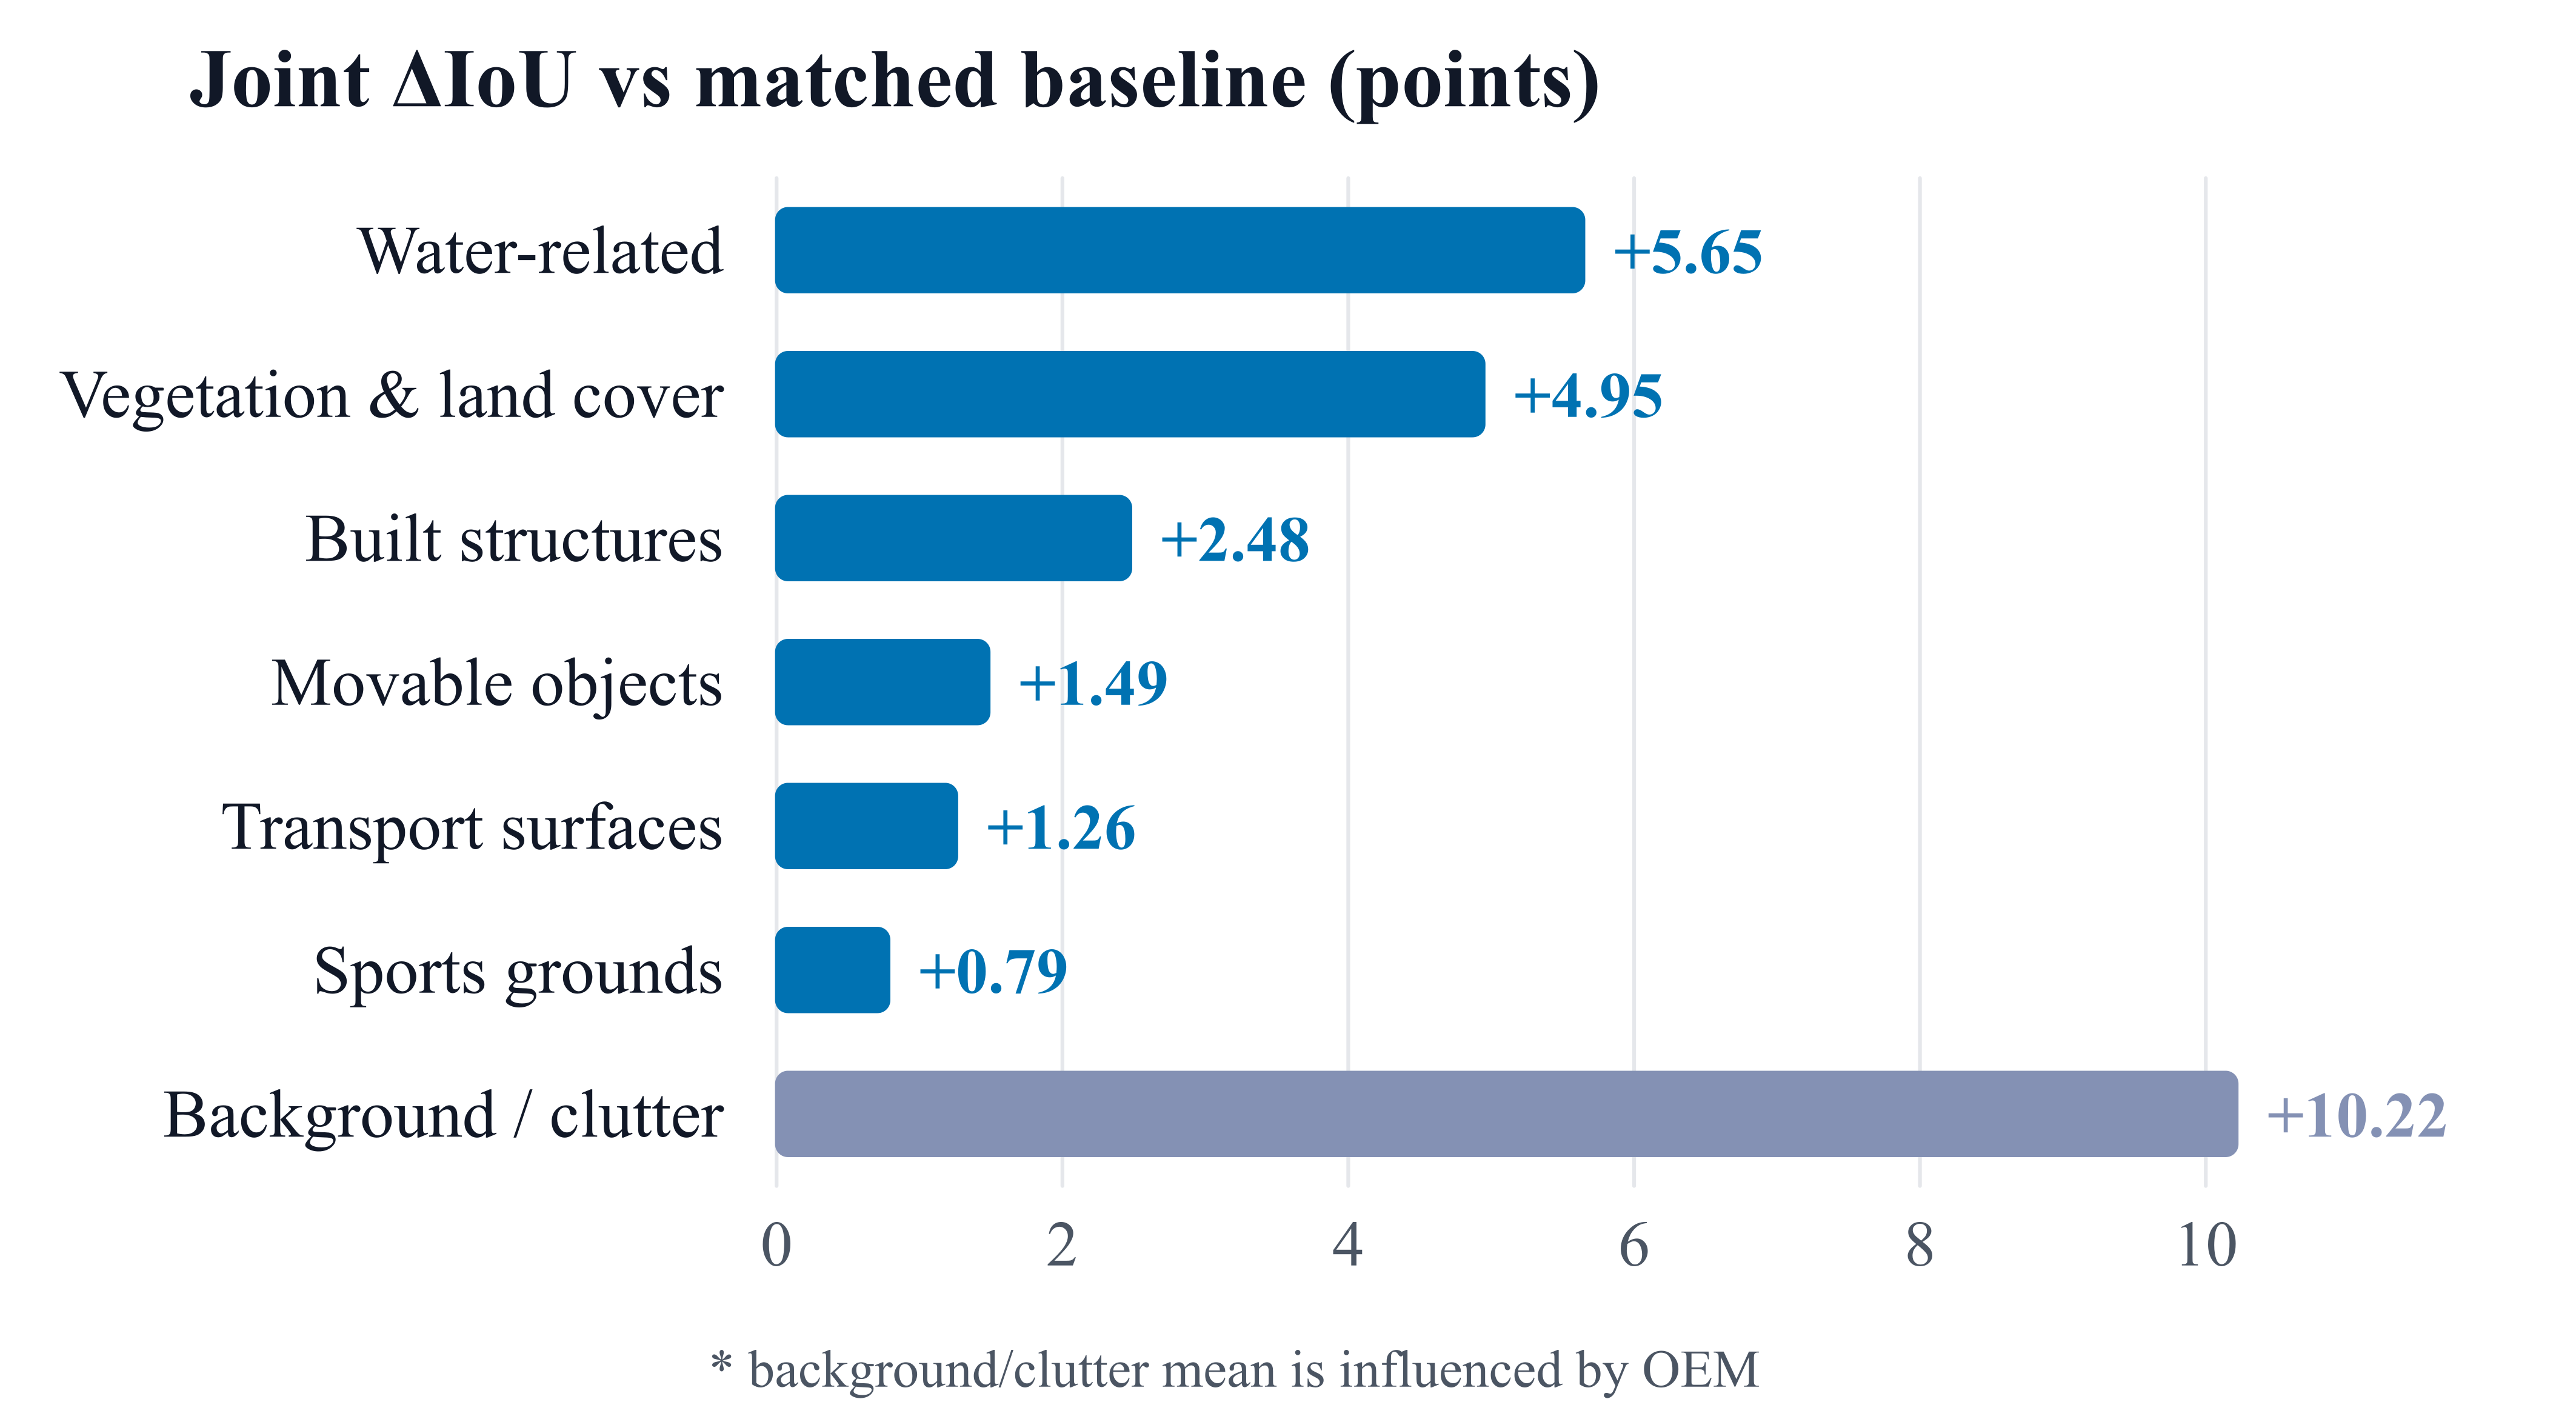
\includegraphics[width=\columnwidth]{fig/category_gain.png}
\caption{Category-group improvements over the matched baseline. The background/clutter mean is influenced by OEM and is shown separately.}
\label{fig:category-gain}
\end{figure}


Figure~\ref{fig:category-gain} summarizes the group-level pattern. JRV improves 48 of 63 dataset--class pairs, including 41 of 55 foreground pairs. Vegetation and land cover show the broadest consistency at 14/15 positive pairs. Water-related and built-structure groups also improve on average. Movable objects receive little average benefit from role text alone ($-0.02$) but improve after joint composition (+1.49), showing that the two stages do not have to benefit the same category groups.

The gains concentrate on classes with weaker baseline performance. The 17 pairs below 30\% baseline IoU improve by +7.03 on average; the 30--60\% group improves by +3.82; the group above 60\% improves by +1.41. This is an average trend, not a monotone guarantee. Transport surfaces are a counterexample: they improve by +1.26 over the baseline but decline by 0.17 relative to role-only prediction. The background/clutter mean is +10.22 and is strongly influenced by OEM; its group median is +1.56, so the foreground results provide the more informative aggregate.

Pixel transitions show that the gains correspond to corrected assignments. Approximately 429.16 million baseline errors become correct, while 165.85 million previously correct pixels become incorrect, a net increase of 263.31 million correct assignments and a correction-to-damage ratio of 2.59. These counts refer to evaluated images and tiles, not independent geographic samples. They complement class-balanced mIoU without implying that every class or component improves.


\begin{center}
\setlength{\fboxsep}{0pt}
\fcolorbox{orange!65!black}{orange!5}{%
\parbox{\dimexpr\columnwidth-2\fboxrule\relax}{%
\centering
\vspace{5pt}
{\bf Qualitative comparison placeholder}\\[3pt]
{\small RGB \quad GT \quad Baseline \quad Role-only \quad View-only \quad Joint}\\[4pt]
{\small\itshape Real masks must be exported for OEM, Vaihingen, UAVid/LoveDA.}\\[5pt]
}}
\captionsetup{hypcap=false}
\captionof{figure}{Placeholder for the qualitative comparison. No prediction or improvement is shown; the panel will be replaced with verified outputs from the fixed profile.}
\label{fig:qualitative-placeholder}
\captionsetup{hypcap=true}
\end{center}

\subsection{Natural-Image Evaluation and Scope}

Natural-image evaluation tests whether role supplementation transfers beyond overhead geometry and remote-sensing ontologies, while keeping the same frozen model and role definitions. VOC20 uses a 20-class foreground vocabulary, and Cityscapes evaluates 19 urban classes under a different scene distribution. We first report the joint result under the same component definitions, then separate the role and view effects.

\begin{center}
\centering
\captionsetup{hypcap=false}
\captionof{table}{Natural-image evaluation (mIoU, \%). Role-only and view-only are separately selected optima; the table is not used to compute interaction. VOC20 uses the foreground vocabulary.}
\label{tab:natural}
\captionsetup{hypcap=true}
\small
\setlength{\tabcolsep}{3pt}
\begin{tabular}{lcccccc}
\toprule
Dataset & Images & Baseline & Role & View & Joint & $\Delta$ \\
\midrule
VOC20~\cite{R44} & 1,449 & 96.89 & 97.00 & 97.00 & \textbf{97.11} & +0.22 \\
Cityscapes~\cite{R43} & 500 & 67.90 & \textbf{72.20} & 68.72 & \textbf{72.20} & +4.29 \\
\bottomrule
\end{tabular}
\end{center}

Role-functional evidence also improves the two natural-image evaluations. VOC20 rises from 96.89 to 97.11, with a small additional view gain and a near-additive interaction (+0.01 after rounding). Cityscapes rises from 67.90 to 72.20, driven by role supplementation. Its joint optimum reduces to the role-specialized Global endpoint, so additional view composition does not improve that endpoint.

The same-image control clarifies the role of observation construction. On Potsdam and Vaihingen, using four 256-pixel crops and a 512-pixel Global view from the current image selects Global in both cases and returns 58.59 and 62.33, respectively, without an additional view gain. The main table instead uses aligned neighboring context for these two datasets. We therefore attribute the large Potsdam and Vaihingen gains to the combined role and observation protocol, not to an arbitrary extra crop. The natural-image results support the transfer of role supplementation while showing that view composition depends on whether the alternative observation yields compatible evidence.

Across the evaluations, the method uses a fixed dataset profile selected offline, freezes all SAM3 weights, and performs no image-level ground-truth routing. These constraints define the evidence: the experiments support role-sensitive evidence organization and conditional view composition under the reported protocols, not universal superiority of shared text, larger fields, or a particular fusion operator.






\section{Conclusion}
\label{sec:conclusion}

We studied how supplementary evidence should enter a frozen concept-grounded segmentation model whose Presence, Semantic, and Instance readouts serve different functions. The central finding is that a shared concept supplies a stable category anchor but does not impose a shared evidence requirement. JRV preserves the official ontology and the native $p\max(S,I)$ path, specializes supplementary text by readout role, and composes aligned Local and Context observations after complete grounding. The eight-benchmark evaluation supports this organization: average mIoU rises from 53.56 to 57.49, every dataset improves over the matched baseline, and the fixed Role--View configuration has positive interaction on six datasets. The category and pixel analyses show that the gain reflects corrected assignments rather than a single dominant class.

The scope is equally part of the result. Dataset-level profiles are selected offline rather than predicted per image, the view operator varies with data distribution, and iSAID and UDD5 exhibit overlapping rather than complementary corrections. Cityscapes selects a Global endpoint, while the same-image Potsdam/Vaihingen control does not support an additional gain from the tested 256/512 crops. These observations position JRV as evidence organization for a frozen concept-grounded model, not as a universal claim that more prompts or larger fields improve segmentation. A natural next step is to replace offline profile selection with a validation-driven or lightweight adaptive policy while preserving the anchor and full-grounding constraints identified here.


\begin{thebibliography}{51}
\providecommand{\natexlab}[1]{#1}
\providecommand{\url}[1]{\texttt{#1}}
\expandafter\ifx\csname urlstyle\endcsname\relax
  \providecommand{\doi}[1]{doi: #1}\else
  \providecommand{\doi}{doi: \begingroup \urlstyle{rm}\Url}\fi

\bibitem{R01}
Alec Radford, Jong~Wook Kim, Chris Hallacy, Aditya Ramesh, Gabriel Goh,
  Sandhini Agarwal, Girish Sastry, Amanda Askell, Pamela Mishkin, Jack Clark,
  Gretchen Krueger, and Ilya Sutskever.
\newblock Learning transferable visual models from natural language
  supervision.
\newblock In \emph{Proceedings of the 38th International Conference on Machine
  Learning}, pages 8748--8763. PMLR, 2021.

\bibitem{R02}
Vladan Stojni\'c, Yannis Kalantidis, Ji\v{r}{\'\i} Matas, and Giorgos Tolias.
\newblock Lposs: Label propagation over patches and pixels for open-vocabulary
  semantic segmentation.
\newblock In \emph{Proceedings of the IEEE/CVF Conference on Computer Vision
  and Pattern Recognition (CVPR)}, pages 9794--9803, 2025.

\bibitem{R03}
Chanyoung Kim, Dayun Ju, Woojung Han, Ming-Hsuan Yang, and Seong~Jae Hwang.
\newblock Distilling spectral graph for object-context aware open-vocabulary
  semantic segmentation.
\newblock In \emph{Proceedings of the IEEE/CVF Conference on Computer Vision
  and Pattern Recognition (CVPR)}, pages 15033--15042, 2025.

\bibitem{R04}
Gensheng Pei, Xiruo Jiang, Xinhao Cai, Tao Chen, Yazhou Yao, and Byeungwoo
  Jeon.
\newblock Pearl: Geometry aligns semantics for training-free open-vocabulary
  semantic segmentation.
\newblock In \emph{Proceedings of the IEEE/CVF Conference on Computer Vision
  and Pattern Recognition (CVPR)}, pages 17927--17937, 2026{\natexlab{a}}.

\bibitem{R05}
Yongkang Li, Tianheng Cheng, Bin Feng, Wenyu Liu, and Xinggang Wang.
\newblock Mask-adapter: The devil is in the masks for open-vocabulary
  segmentation.
\newblock In \emph{Proceedings of the IEEE/CVF Conference on Computer Vision
  and Pattern Recognition (CVPR)}, pages 14998--15008, 2025{\natexlab{c}}.

\bibitem{R06}
Kaiyu Li, Ruixun Liu, Xiangyong Cao, Xueru Bai, Feng Zhou, Deyu Meng, and Zhi
  Wang.
\newblock Segearth-ov: Towards training-free open-vocabulary segmentation for
  remote sensing images.
\newblock In \emph{Proceedings of the IEEE/CVF Conference on Computer Vision
  and Pattern Recognition (CVPR)}, pages 10545--10556, 2025{\natexlab{a}}.

\bibitem{R07}
Xin Niu, Manqi Zhao, Dongsheng Jiang, Yingying Wu, and Bing Su.
\newblock Reattnclip: Training-free open-vocabulary remote sensing image
  segmentation via re-defined attention in clip.
\newblock In \emph{Proceedings of the IEEE/CVF Conference on Computer Vision
  and Pattern Recognition (CVPR)}, pages 24980--24989, 2026.

\bibitem{R08}
Ting Yang, Qilong Wang, Qibin Hou, and Qinghua Hu.
\newblock Test-time multi-prompt adaptation for open-vocabulary remote sensing
  image segmentation.
\newblock In \emph{Proceedings of the IEEE/CVF Conference on Computer Vision
  and Pattern Recognition (CVPR)}, pages 10699--10709, 2026.

\bibitem{R09}
Gensheng Pei, Xiruo Jiang, Yazhou Yao, Xiangbo Shu, Fumin Shen, and Byeungwoo
  Jeon.
\newblock Taming {SAM3} in the wild: A concept bank for open-vocabulary
  segmentation.
\newblock \emph{arXiv preprint arXiv:2602.06333}, 2026{\natexlab{b}}.

\bibitem{R10}
Nicolas Carion et~al.
\newblock {SAM 3}: Segment anything with concepts.
\newblock \emph{arXiv preprint arXiv:2511.16719}, 2025.

\bibitem{R11}
Kaiyu Li, Shengqi Zhang, Yujie Wang, Yupeng Deng, Zhi Wang, Deyu Meng, and
  Xiangyong Cao.
\newblock {SegEarth-OV3}: Exploring {SAM 3} for open-vocabulary semantic
  segmentation in remote sensing images.
\newblock \emph{arXiv preprint arXiv:2512.08730}, 2025{\natexlab{b}}.

\bibitem{R12}
Yanghui Song, Nanqing Liu, Haonan Yin, Yingjie Gao, Chengfu Yang, and Qi Ming.
\newblock Prompt-calibrated {SAM 3} for open-vocabulary remote sensing semantic
  segmentation.
\newblock \emph{arXiv preprint arXiv:2606.21863}, 2026.

\bibitem{R13}
Yanhui Chen, Baoyao Yang, Siqi Liu, and Jingchao Wang.
\newblock {CoCo-SAM3}: Harnessing concept conflict in open-vocabulary semantic
  segmentation.
\newblock \emph{arXiv preprint arXiv:2604.19648}, 2026{\natexlab{c}}.

\bibitem{R14}
ByeongCheol Lee, Hyun~Seok Seong, Sangeek Hyun, Gilhan Park, WonJun Moon, and
  Jae-Pil Heo.
\newblock Looking beyond the window: Global-local aligned clip for
  training-free open-vocabulary semantic segmentation.
\newblock In \emph{Proceedings of the IEEE/CVF Conference on Computer Vision
  and Pattern Recognition (CVPR)}, pages 27686--27696, 2026.

\bibitem{R15}
Seungjae Moon, Seunghyun Oh, and Youngmin Ro.
\newblock {OV-Stitcher}: A global context-aware framework for training-free
  open vocabulary semantic segmentation.
\newblock In \emph{Proceedings of the IEEE/CVF Conference on Computer Vision
  and Pattern Recognition (CVPR) Findings}, pages 7357--7367, 2026.

\bibitem{R16}
Ziyu Zhao, Xiaoguang Li, Lingjia Shi, Nasrin Imanpour, and Song Wang.
\newblock Dpseg: Dual-prompt cost volume learning for open-vocabulary semantic
  segmentation.
\newblock In \emph{Proceedings of the IEEE/CVF Conference on Computer Vision
  and Pattern Recognition (CVPR)}, pages 25346--25356, 2025.

\bibitem{R17}
Jianjian Yin, Tao Chen, Yi Chen, Gensheng Pei, Xiangbo Shu, Yazhou Yao, and
  Fumin Shen.
\newblock Pca-seg: Revisiting cost aggregation for open-vocabulary semantic and
  part segmentation.
\newblock In \emph{Proceedings of the IEEE/CVF Conference on Computer Vision
  and Pattern Recognition (CVPR)}, pages 27633--27643, 2026.

\bibitem{R18}
Lukas Hoyer, Dengxin Dai, and Luc Van~Gool.
\newblock {HRDA}: Context-aware high-resolution domain-adaptive semantic
  segmentation.
\newblock In \emph{European Conference on Computer Vision (ECCV)}, 2022.

\bibitem{R19}
Hengzhi Chen, Liqian Feng, Wenhua Wu, Xiaogang Zhu, Qiuxia Wu, Lianlei Shan,
  and Kun Hu.
\newblock F2net: A frequency-fused network for ultra-high resolution remote
  sensing segmentation.
\newblock In \emph{Proceedings of the IEEE/CVF Conference on Computer Vision
  and Pattern Recognition (CVPR)}, pages 13275--13284, 2026{\natexlab{a}}.

\bibitem{R20}
Mingjie Xie, Guangjun He, Dongli Xu, Youtian Lin, Hongjue Li, Pengming Feng,
  Jian Guan, and Yue Deng.
\newblock Synclip: Synonym-coherent language-image pretraining for robust
  open-vocabulary dense perception.
\newblock In \emph{Proceedings of the IEEE/CVF Conference on Computer Vision
  and Pattern Recognition (CVPR)}, pages 31524--31533, 2026.

\bibitem{R21}
Qi Zhu, Jiangwei Lao, Deyi Ji, Junwei Luo, Kang Wu, Yingying Zhang, Lixiang Ru,
  Jian Wang, Jingdong Chen, Ming Yang, Dong Liu, and Feng Zhao.
\newblock Skysense-o: Towards open-world remote sensing interpretation with
  vision-centric visual-language modeling.
\newblock In \emph{Proceedings of the IEEE/CVF Conference on Computer Vision
  and Pattern Recognition (CVPR)}, pages 14733--14744, 2025.



\bibitem{R22}
Yimin Wei, Aoran Xiao, Hongruixuan Chen, Junshi Xia, and Naoto Yokoya.
\newblock Mm-ovseg: Multimodal optical-sar fusion for open-vocabulary
  segmentation in remote sensing.
\newblock In \emph{Proceedings of the IEEE/CVF Conference on Computer Vision
  and Pattern Recognition (CVPR)}, pages 42202--42212, 2026.

\bibitem{R23}
Yunxiang Fu, Meng Lou, and Yizhou Yu.
\newblock Segman: Omni-scale context modeling with state space models and local
  attention for semantic segmentation.
\newblock In \emph{Proceedings of the IEEE/CVF Conference on Computer Vision
  and Pattern Recognition (CVPR)}, pages 19077--19087, 2025.

\bibitem{R24}
Mohammad Dabaja and Turgay Celik.
\newblock Promptable concept segmentation from above: Evaluating sam 3's
  zero-shot and one-shot capabilities in remote sensing.
\newblock \emph{arXiv preprint arXiv:2607.09583}, 2026.

\bibitem{R25}
Shanwen Wang, Xin Sun, Sirui Wang, and Xiao~Xiang Zhu.
\newblock Rsgpnet: Geometric prompting for remote sensing open-vocabulary
  semantic segmentation.
\newblock \emph{arXiv preprint arXiv:2606.28410}, 2026.

\bibitem{R26}
Wenyang Chen, Zhanxuan Hu, Yaping Zhang, Hailong Ning, and Yonghang Tai.
\newblock Coninfer: Context-aware inference for training-free open-vocabulary
  remote sensing segmentation.
\newblock In \emph{Proceedings of the IEEE/CVF Conference on Computer Vision
  and Pattern Recognition (CVPR) Findings}, 2026{\natexlab{b}}.

\bibitem{R27}
Changhao Zhao, Haoxiang Li, Yuke Li, Hai Liu, and LingLin Zeng.
\newblock Standalone dinov3 for remote sensing training-free open-vocabulary
  semantic segmentation.
\newblock \emph{arXiv preprint arXiv:2608.03023}, 2026.

\bibitem{R28}
Mohammadreza Heidarianbaei, Mareike Dorozynski, Hubert Kanyamahanga, Max
  Mehltretter, and Franz Rottensteiner.
\newblock Open-vocabulary semantic segmentation in remote sensing via
  hierarchical attention masking and model composition.
\newblock \emph{arXiv preprint arXiv:2602.23869}, 2026.

\bibitem{R29}
Feng Wang, Jieru Mei, and Alan Yuille.
\newblock {SCLIP}: Rethinking self-attention for dense vision-language inference.
\newblock In \emph{European Conference on Computer Vision (ECCV)}, pages
  315--332, 2024.
\newblock \doi{10.1007/978-3-031-72664-4_18}

\bibitem{R30}
Mengcheng Lan, Chaofeng Chen, Yiping Ke, Xinjiang Wang, Litong Feng, and
  Wayne Zhang.
\newblock {ClearCLIP}: Decomposing {CLIP} representations for dense
  vision-language inference.
\newblock In \emph{European Conference on Computer Vision (ECCV)}, pages
  143--160, 2024.
\newblock \doi{10.1007/978-3-031-72970-6_9}

\bibitem{R31}
Mengcheng Lan, Chaofeng Chen, Yiping Ke, Xinjiang Wang, Litong Feng, and
  Wayne Zhang.
\newblock {ProxyCLIP}: Proxy attention improves {CLIP} for open-vocabulary
  segmentation.
\newblock In \emph{European Conference on Computer Vision (ECCV)}, pages
  70--88, 2024.
\newblock \doi{10.1007/978-3-031-73113-6_5}

\bibitem{R32}
Hao Zhu, Shuo Jin, Wenbin Liao, Jiayu Xiao, Yan Zhu, Siyue Yu, and Feng Dai.
\newblock {VIP}: Visual-guided prompt evolution for efficient dense
  vision-language inference.
\newblock In \emph{Proceedings of the International Conference on Machine
  Learning (ICML)}, 2026.

\bibitem{R33}
Shanwen Wang, Xin Sun, Jungong Han, and Xiao~Xiang Zhu.
\newblock {RSCLIP} for training-free open-vocabulary remote sensing image
  semantic segmentation.
\newblock \emph{IEEE Journal of Selected Topics in Applied Earth Observations
  and Remote Sensing}, 19:15626--15639, 2026.
\newblock \doi{10.1109/JSTARS.2026.3688939}

\bibitem{R34}
Dengke Zhang, Fagui Liu, and Quan Tang.
\newblock {CorrCLIP}: Reconstructing patch correlations in {CLIP} for
  open-vocabulary semantic segmentation.
\newblock In \emph{Proceedings of the IEEE/CVF International Conference on
  Computer Vision (ICCV)}, pages 24677--24687, 2025.
\newblock \doi{10.1109/ICCV51701.2025.02288}

\bibitem{R35}
Tran~Dinh Tien and Zhiqiang Shen.
\newblock {ActiveSAM}: Fast and accurate open-vocabulary semantic
  segmentation with frozen {SAM}~3.
\newblock \emph{arXiv preprint arXiv:2606.16996}, 2026.

\bibitem{R36}
Junjue Wang, Zhuo Zheng, Ailong Ma, Xiaoyan Lu, and Yanfei Zhong.
\newblock {LoveDA}: A remote sensing land-cover dataset for domain adaptive
  semantic segmentation.
\newblock In \emph{Proceedings of the Neural Information Processing Systems
  Track on Datasets and Benchmarks}, volume~1, 2021.

\bibitem{R37}
Syed~Waqas Zamir, Aditya Arora, Akshita Gupta, Salman Khan, Guolei Sun,
  Fahad~Shahbaz Khan, Fan Zhu, Ling Shao, Gui-Song Xia, and Xiang Bai.
\newblock {iSAID}: A large-scale dataset for instance segmentation in aerial
  images.
\newblock In \emph{Proceedings of the IEEE/CVF Conference on Computer Vision
  and Pattern Recognition Workshops (CVPRW)}, 2019.

\bibitem{R38}
Junshi Xia, Naoto Yokoya, Bruno Adriano, and Clifford Broni-Bediako.
\newblock {OpenEarthMap}: A benchmark dataset for global high-resolution land
  cover mapping.
\newblock In \emph{Proceedings of the IEEE/CVF Winter Conference on
  Applications of Computer Vision (WACV)}, pages 6243--6253, 2023.
\newblock \doi{10.1109/WACV56688.2023.00619}

\bibitem{R39}
Ye Lyu, George Vosselman, Gui-Song Xia, Alper Yilmaz, and Michael~Ying Yang.
\newblock {UAVid}: A semantic segmentation dataset for {UAV} imagery.
\newblock \emph{ISPRS Journal of Photogrammetry and Remote Sensing},
  165:108--119, 2020.
\newblock \doi{10.1016/j.isprsjprs.2020.05.009}

\bibitem{R40}
Yu Chen, Yao Wang, Peng Lu, Yisong Chen, and Guoping Wang.
\newblock Large-scale structure from motion with semantic constraints of aerial
  images.
\newblock In \emph{Pattern Recognition and Computer Vision (PRCV)}, pages
  347--359, 2018.
\newblock \doi{10.1007/978-3-030-03398-9_30}

\bibitem{R41}
Wenxiao Cai, Ke Jin, Jinyan Hou, Cong Guo, Letian Wu, and Wankou Yang.
\newblock {VDD}: Varied drone dataset for semantic segmentation.
\newblock \emph{Journal of Visual Communication and Image Representation},
  109:104429, 2025.
\newblock \doi{10.1016/j.jvcir.2025.104429}

\bibitem{R42}
\newblock {ISPRS} 2D semantic labeling benchmark: Potsdam and Vaihingen.
\newblock International Society for Photogrammetry and Remote Sensing.
\newblock \url{https://www.isprs.org/education/benchmarks/UrbanSemLab/}

\bibitem{R43}
Marius Cordts, Mohamed Omran, Sebastian Ramos, Timo Rehfeld, Markus
  Enzweiler, Rodrigo Benenson, Uwe Franke, Stefan Roth, and Bernt Schiele.
\newblock The {Cityscapes} dataset for semantic urban scene understanding.
\newblock In \emph{Proceedings of the IEEE/CVF Conference on Computer Vision
  and Pattern Recognition (CVPR)}, pages 3213--3223, 2016.
\newblock \doi{10.1109/CVPR.2016.350}

\bibitem{R44}
Mark Everingham, Luc Van~Gool, Christopher~K.~I. Williams, John Winn, and
  Andrew Zisserman.
\newblock The {PASCAL} visual object classes ({VOC}) challenge.
\newblock \emph{International Journal of Computer Vision}, 88(2):303--338,
  2010.
\newblock \doi{10.1007/s11263-009-0275-4}

\bibitem{R45}
Jiarui Xu, Shalini De~Mello, Sifei Liu, Wonmin Byeon, Thomas Breuel, Jan
  Kautz, and Xiaolong Wang.
\newblock {GroupViT}: Semantic segmentation emerges from text supervision.
\newblock In \emph{Proceedings of the IEEE/CVF Conference on Computer Vision
  and Pattern Recognition (CVPR)}, pages 18113--18123, 2022.
\newblock \doi{10.1109/CVPR52688.2022.01760}

\bibitem{R46}
Feng Liang, Bichen Wu, Xiaoliang Dai, Kunpeng Li, Yinan Zhao, Hang Zhang,
  Peizhao Zhang, Peter Vajda, and Diana Marculescu.
\newblock Open-vocabulary semantic segmentation with mask-adapted {CLIP}.
\newblock In \emph{Proceedings of the IEEE/CVF Conference on Computer Vision
  and Pattern Recognition (CVPR)}, pages 7061--7070, 2023.
\newblock \doi{10.1109/CVPR52729.2023.00682}

\bibitem{R47}
Yuhang Yang, Jinhong Deng, Wen Li, and Lixin Duan.
\newblock {ResCLIP}: Residual attention for training-free dense
  vision-language inference.
\newblock In \emph{Proceedings of the IEEE/CVF Conference on Computer Vision
  and Pattern Recognition (CVPR)}, pages 29968--29978, 2025.
\newblock \doi{10.1109/CVPR52734.2025.02789}

\bibitem{R48}
Seokju Cho, Heeseong Shin, Sunghwan Hong, Anurag Arnab, Paul~Hongsuck Seo,
  and Seungryong Kim.
\newblock {CAT-Seg}: Cost aggregation for open-vocabulary semantic
  segmentation.
\newblock In \emph{Proceedings of the IEEE/CVF Conference on Computer Vision
  and Pattern Recognition (CVPR)}, pages 4113--4123, 2024.
\newblock \doi{10.1109/CVPR52733.2024.00394}

\bibitem{R49}
Bin Xie, Jiale Cao, Jin Xie, Fahad~Shahbaz Khan, and Yanwei Pang.
\newblock {SED}: A simple encoder-decoder for open-vocabulary semantic
  segmentation.
\newblock In \emph{Proceedings of the IEEE/CVF Conference on Computer Vision
  and Pattern Recognition (CVPR)}, pages 3426--3436, 2024.
\newblock \doi{10.1109/CVPR52733.2024.00329}

\bibitem{R50}
Yu Hu, Jianyang Gu, Hao Liu, Yue Cao, Jozsef Hamari, Zheng Liu, and Mohsen
  Zardadi.
\newblock {AVION}: Aerial vision-language instruction from offline teacher to
  prompt-tuned network.
\newblock In \emph{Proceedings of the IEEE/CVF Conference on Computer Vision
  and Pattern Recognition (CVPR)}, 2026.

\bibitem{R51}
Bingfeng Zhang, Siyue Yu, Hui Li, Jiahua Lin, Wenwu Wang, and Jimin Xiao.
\newblock The power of prior: Training-free open-vocabulary semantic
  segmentation with {LLaVA}.
\newblock In \emph{Proceedings of the IEEE/CVF Conference on Computer Vision
  and Pattern Recognition (CVPR)}, 2026.

\end{thebibliography}




\end{document}



